\label{chap:LCA}
\section{\acl{LCA} Framework}
\label{chap:LCA-framework}
To understand \acf{LCA} databases, the framework of \ac{LCA} is presented. \ac{LCA} is a systematic procedure to assess the impact of a product on the environment. The impacts are assessed throughout the whole life cycle of the product: the product life cycle starts with raw material extraction from the environment, continues with production, transport, use, maintenance, end of life treatment and ends with final disposal or recycling \cite{InternationalOrganizationforStandardization.2006}.

\subsection{Phases of \acl{LCA}}
A \ac{LCA} study consists of four phases. Going through the four phases is not a linear but an iterative process. Results from one phase may show that refinements are needed. Possibly, those refinements have to be made in previous \ac{LCA} phases  \cite{InternationalOrganizationforStandardization.2006}. The next paragraphs introduce the four phases of \ac{LCA}.

\paragraph{Phase 1: Goal and scope definition} The first step is to define the reason for conducting the \ac{LCA} study. Furthermore, the target audience is identified. The scope defines the product system and its functions that are studied. The function of the product is quantified in a functional unit. In chemical \acp{LCA}, the functional unit is 1 kg of the produced chemical. Defining the system requires a decision on which of the life cycle stages and processes are included in the study. Additionally, to ensure that the results comply with the goal, quality requirements for utilized data have to be set. Moreover, to obtain transparency and consistency, all assumptions made have to be documented in the scope definition %Documenting assumptions is an example for the iterative nature of \ac{LCA}: Whenever later in the procedure a decision requires assumptions, it is necessary to return to the scope definition to document it
 \cite{InternationalOrganizationforStandardization.2006}.

\paragraph{Phase 2: Life Cycle Inventory Analysis} In each life cycle stage, flows of mass or energy pass the system boundary of the product system under study. Flows can be exchanged with the technosphere or with the natural environment \cite{InternationalOrganizationforStandardization.2006}. Flows exchanged with the technosphere are called technical flows, whereas flows to and from the natural environment are called elementary flows. Examples for technical flows are products, intermediates, ancillary inputs or energy; examples for elementary flows are raw materials, landfilled wastes or emissions. In contrast to technical flows, elementary flows have a potential direct impact on the natural environment. Still, technical flows of a system have an environmental effect outside of the product system, as supplying the technical flows result in elementary flows from and to the supply systems.% The foreground system is the system under study, while the background system is the set of systems supplying the foreground system with technical flows. Thus, the elementary flows or derived impacts of the background system have to be added to the foreground system.

In the Life Cycle Inventory Analysis phase, the \ac{LCA} practitioner collects and lists all elementary and  technical flows that cross the system boundary defined in the scope. Consequentially, all flows are related to the functional unit. In the relative format, the data is called inventory. The smallest component for which inventory information is compiled is called unit process \cite{InternationalOrganizationforStandardization.2006b}. Additionally, in the Life Cycle Inventory Analysis phase the quality of data is validated \cite{InternationalOrganizationforStandardization.2006}.
%Sources for flows crossing the system boundary can be found in scientific literature, process descriptions or patents. For LCA of chemical processes, flows can be taken from plant data, process simulation or different process design methods. Listing all relevant flows consumes much time and resouces  \cite{Parvatker.2019}. This work aims to facilitate Life Cycle Inventory Analysis for chemical processes by deeper understanding the consequences of using \acl{spdm}s for the calculation of elementary and technical flows.

\paragraph{Phase 3: \acl{LCIA}} The idea of \acf{LCIA} is that elementary flows can be categorized according to their impact on the environment.  This categorization can be done, because several flows have a similar impact on the environment. For example, elementary flows of carbon dioxide, dinitrogen oxide and methane contribute to the same environmental impact: global warming. Examples for impact categories are global warming impact, terrestrial ecosystem damage, human toxicity, radiation, acidification, freshwater eutrophication and land use  \cite{Huijbregts.2016}. Every impact category is represented by an indicator. The indicator is an elementary flow of a representative substance that is equivalent to the sum of all elementary flows of different substances that contribute to the impact category \cite{InternationalOrganizationforStandardization.2006b}. For instance, the global warming impact indicator is mass of CO$_2$ equivalent.
%International Standard ISO 14040 \cite{InternationalOrganizationforStandardization.2006} requires a procedure of mandatory steps to perform a \ac{LCIA}: First the LCA practitioner chooses relevant impact categories to consider.  Then the LCI results are assigned to impact categories, the LCI results contribute to (classification).  Finally the category indicator is calculated (characterization): 
Depending on the substance, elementary flows contribute differently to the impact category. The contribution to an impact category is modeled by a characterization factor. For each impact category, elementary flows are multiplied with the characterization factors, resulting in an equivalent elementary flow. Adding the equivalent elementary flows yields the impact category indicator \cite{InternationalOrganizationforStandardization.2006b}.
%It is challenging, to define objective characterization factors. For instance characterization factors for global warming impact of green house gases differ depending on the timescale considered. Thus LCA
Usually, practitioners rely on existing \ac{LCIA} methodologies from publications that include ready-to-use characterization factors \cite{InternationalOrganizationforStandardization.2006b}.

\paragraph{Phase 4: Life cycle interpretation} This phase evaluates the results of the LCA. With a contribution analysis, significant issues are identified. Significant issues are processes or life cycle stages that contribute overproportionally to the final result. Furthermore, a multitude of methods can increase confidence in the result of the LCA study. A sensitivity check reveals how robust the results of the study are against made assumptions and uncertainties in data. A consistency check analyses if assumptions, methods and data used in the LCA are consistent with the goal and scope of the study. Finally, findings and limitations of the study are summarized and conclusions are drawn. Based on the conclusions, recommendations are derived and documented  \cite{InternationalOrganizationforStandardization.2006b}.

\subsection{Methodological Choices in \acl{LCA}}
\label{multi-output}

\begin{figure}[h]
    \centering
    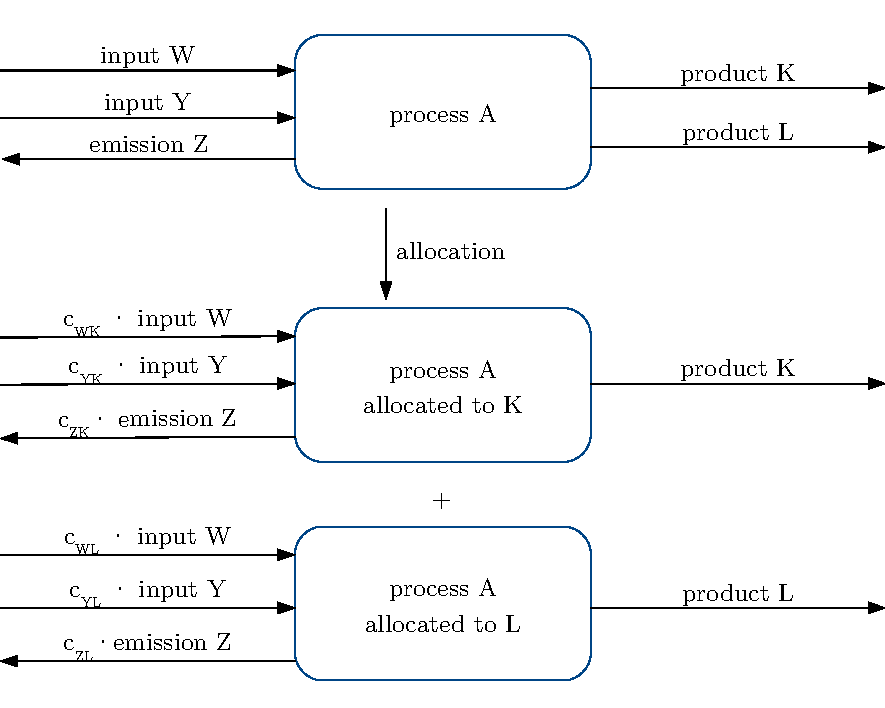
\includegraphics[]{images/allocation.pdf}
    \caption[Allocation]{Allocation is one attempt to solve the multi-output problem in LCA. In this example, process A has two product outputs: K and L. To assign the input flows W, Y and the emission Z to the product flows, the input flows and emissions are partitioned with allocation factors $c_{WK}$, $c_{YK}, c_{ZK}, c_{WL}, c_{YL}$ and $c_{ZL}$. Allocation factors are based on mass, energy or economic price of the output products \cite{InternationalOrganizationforStandardization.2006}. For chemical processes, inputs can be educts, heat or electricity.}
    \label{fig:allocation}
\end{figure}

Conducting a LCA brings some challenges. Chapter \ref{multi-output} presents typical issues and common practices to solve the challenges. Furthermore, to understand LCA database results, this chapter analyses how methodological choices influence the LCA database results. In this thesis, LCA database results are defined as a database of life cycle inventories or impacts of products. This thesis focuses on the methodological choices allocation and cut-off.


\paragraph{Multi-output problem} In general, industrial processes produce numerous products. Inevitably, to run the process, numerous input flows are necessary. Also, a variety of emissions and wastes are produced. Hence, an inventory for the process would have several products. However, LCA practitioners are interested in the inventory per functional unit, which often is related to the product instead of the process. In this case, the practitioner needs to assign the inventory to the products \cite{InternationalOrganizationforStandardization.2006}. The subsequent paragraphs present two approaches to handle the multi-output problem.

\paragraph{System expansion}In order to solve the multi-output problem, ISO 14040 \cite{InternationalOrganizationforStandardization.2006} recommends to expand the product system and to include all product outputs of the process into the functional unit. However, in some cases, this may not align with the goal of the LCA study.

\paragraph{Allocation}
Figure \ref{fig:allocation} illustrates the procedure of allocation. In the allocation approach, the process inputs, emissions and waste flows are mathematically partitioned between all product outputs of the process. Partitioning the flows can be based on the relation of mass, energy or economic prices of the products  \cite{InternationalOrganizationforStandardization.2006}.



\paragraph{Implications of Allocation} With the tools of natural science, it is only possible to quantify inventories of a multi-output process. However, allocating the result to a product requires to partition the inventory. Because the inventory is only defined for the process, there is no objective right way to allocate. Furthermore, partitioning always is a value choice how to choose the allocation factor. When doing allocation based on mass, energy or price, in general the inventories differ. Thus, the allocation factor influences the LCA database results.

Chlorine production is an example for how implementing allocation introduces challenges into the LCA. Chlorine is produced in the chlor-alkali process, a decomposition of sodium chloride solution into chlorine, sodium hydroxide solution and hydrogen  \cite{Du.2018}. Thus, to build an inventory of chlorine, allocation to the three products is performed. First energy allocation based on the enthalpy of formation is considered: elements have a standard enthalpy of formation of zero. In the chlorine example, the allocation factor of chlorine and hydrogen is zero, because they are elements. Thus, all inventories and impacts of the process and its supply are allocated to sodium hydroxide. Considering energy allocation based on the heating value instead for allocation is suitable for hydrogen. However, chlorine and sodium hydroxide are typically not burned for energy production. Thus, this attempt is not applicable here.

In a second attempt, allocation based on mass is chosen. In the process, hydrogen, sodium hydroxide and chlorine are formed in the mass ratios 1.3 \%, 52 \% and 46 \% \cite{Hischier.}. Thus, in this example, allocation based on mass results in a complete different result compared to allocation based on energy.

As mentioned in the introduction (Chapter 1), there are methods to calculate the life cycle inventory of chemical processes. In general, these methods are afflicted with errors. In particular, the amounts of output products a process are erroneous. When allocating the flows to the products based on mass, the error of the output masses propagates to all other flows in the inventory.

\paragraph{Cut-off}
LCA practitioners face the problem of a vast amount of inventory data to collect. Therefore, cut-off is implemented to reduce data requirement. Inventory flows, which have a minor contribution to the LCA result are excluded from the inventory. To distinguish which flowss are relevant in practice, a threshold can be defined. The threshold can be a share of mass or energy of the inventory. Then, all the largest flows, which contribute together as much as the threshold of the inventory,  are considered in the inventory. The smaller flows are cut-off. Also, a cut-off criterion based on environmental significance can be defined. In any case, the cut-off criterion has to be documented in the scope definition of the LCA \cite{InternationalOrganizationforStandardization.2006b}.
 
\paragraph{Implications of cut-off}  When the LCA excludes mass flows, the inventory gets smaller. Thus, the LCIA result is rather underestimated; in any case, never overestimated. When the cut-off is done properly, the implications are minor. To do the cut-off properly, there are critical flows to consider. Even small amounts of critical flows can contribute significantly to the LCIA result. Possibly, the mass flow is below the cut-off limit, but has a relevant impact nevertheless. To prevent an underestimation of LCIA results because of cut-off of critical flows, special care has to be taken.
%Additionally, it has to be considered that cut-off changes the system boundary \cite{InternationalOrganizationforStandardization.2006b}.

\section{\acl{LCA} Database Structures}

\begin{figure}[h!]
    \centering
    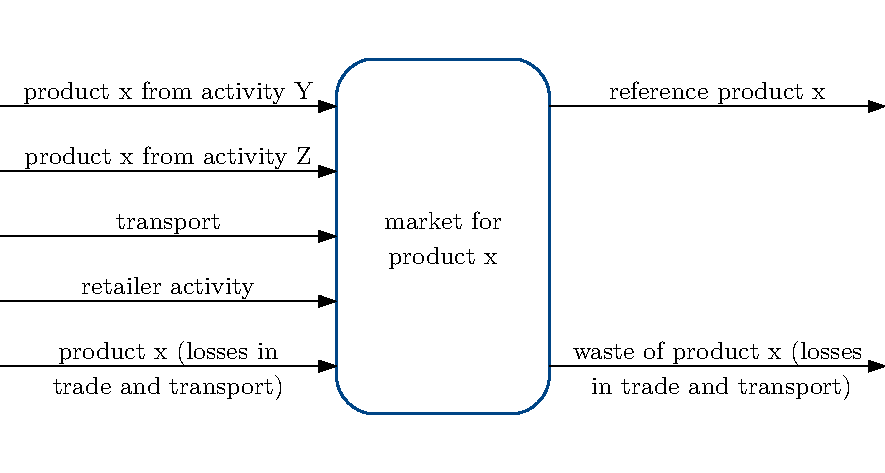
\includegraphics[]{images/market-dataset.pdf}
    \caption[Market dataset in Ecoinvent]{Market dataset in Ecoinvent version 3, which is defined by its name and its inputs and outputs. Adapted from \url{https://www.ecoinvent.org/files/faq_-_market_activity_ecoinvent_3.png}, accessed on March 14, 2020.}
    \label{fig:market}
\end{figure}
\ac{LCA} databases help LCA practitioners to find life cycle inventories or impacts. Thus, databases play an important role in LCA \cite{Wernet.2016}. To understand how  LCA databases are affected by using \aclp{spdm}, this chapter analyses LCA database structure and  generation as well as how LCA database results are affected by the database structure. The LCA database structures are explained on the example of Ecoinvent \cite{Ecoinvent.2020}, a commercial LCA database.

In this thesis, the entries of inventories or impacts for a multitude of chemicals, which are organized in a database, are described by ``LCA database results''. The model of the production network that is used to generate the LCA database results, is described by ``production network model''. LCA database results and the production network model together are described by LCA database. 

The structure of the Ecoinvent database reflects this distinction. Ecoinvent consists of several database layers. In the consumer interface layer, the database customer can access life cycle inventories or impacts results of products. In a second layer, the database calculation layer, life cycle inventories are calculated  \cite{Frischknecht.2007}.

\begin{figure}
    \centering
    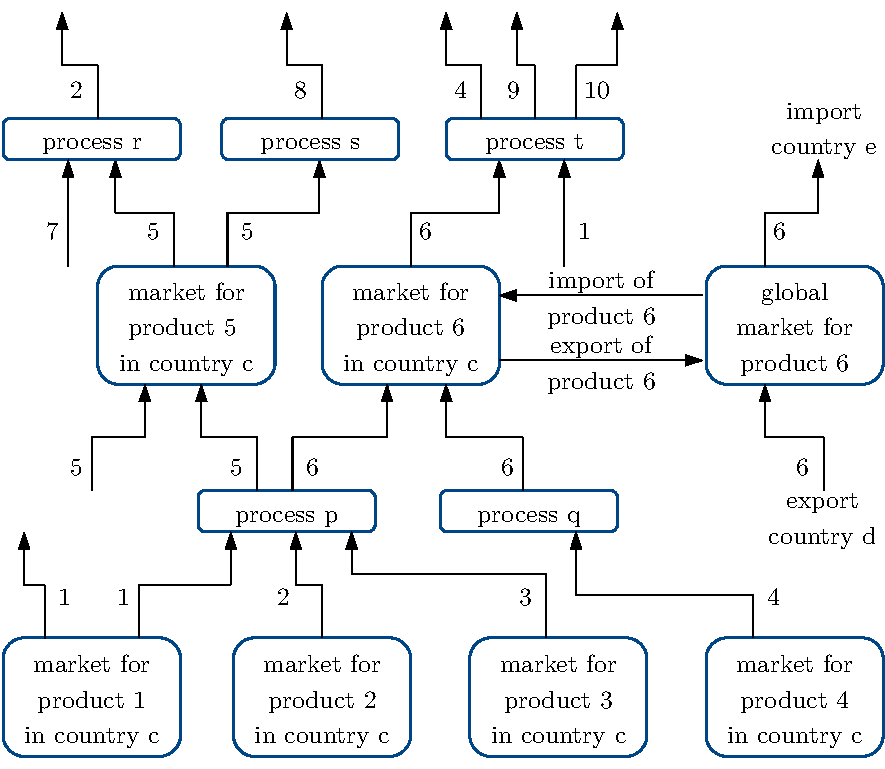
\includegraphics{images/LCA-database.pdf}
    \caption[Production network model]{The production network consists of interconnected production and trade activities that form a global network. This schematic illustration only accounts for the part of the network that is located in country c. The processes p...t each transform  educts into products, wastes and emissions. To keep overview, waste and emission are not depicted. Also, only one global market is depicted, even though all products are traded globally.}
    \label{fig:production-network}
\end{figure}

\paragraph{Production network model}LCA databases model the production network.  This network consists of production activities that are interconnected with each other via intermediates. Each production  activity produces intermediates that are educts for different consecutive production activities. Furthermore, production activities happen in different countries that trade products and intermediates, expanding the network to global size. The sum of all production and trade activities together form a dense network of activities. After several steps, the output of the production network are the final products.

\paragraph{Production activities}All activities in Ecoinvent are represented by datasets with input, output and the name of the activity \cite{Wernet.2016}. Examples for activities are production, transport or market. Production activities are represented by production datasets. Characteristically, chemical production datasets have different inputs and outputs, because a reaction takes place that transforms educts into products.

\paragraph{Market activities}
When modeling a production network, it is important to consider the contribution of a specific production activity to the supply chain. This is necessary in two cases: first, if a product is produced by several production technologies, and second, if the production happens in more than one region. In Ecoinvent, market activities implement both considerations. Figure \ref{fig:market} illustrates the structure of a market dataset in Ecoinvent. Market dataset consists of several inputs and outputs: inputs are flows of the product x from the activity W, Y, Z as well as for compensation of losses in transport;  additional inputs are activities of the retailer. The reference product x and losses from trade and transport are listed as outputs of the market datasets in Ecoinvent. Examples for losses during transport and trade are electrical losses in electricity wires or leakages in chemical pipelines  \cite{Wernet.2016}.  The share of production activities W, Y, Z is named production mix.

The production network is modeled based on consumption mixes. Each educt necessary for a production activity is a mixture of equal educt substances, which are of regional and imported origin.  The consumption mix is calculated by adding the production and import, followed by subtracting the export \cite{Wernet.2016}. The consumption has to be calculated separately for every geographic region that is included. This calculation is based on the assumption that the amount of stored products in the geographic area is stationary in time. In this thesis, consumption mixes are also called market mixes.

\paragraph{Implications of production mixes and consumption mixes for generating LCA databases}

Implications for inventories or impacts occur from the quality of production mix and market mix data: if a product is produced by several technologies with highly different impacts, the accuracy of production mix and market mix data strongly influences the  LCIA result. For example,  the life cycle impact of electricity differs depending on the geographic region. Thus, the impact of the same technology may significantly differ from one region with a large share of renewable energy to a region with a large share of fossil generated electricity. For production technologies with similar impacts, uncertainties in production mix and market mix data have smaller influences.

\paragraph{Regional coverage}
Reasons to implement regional geographical coverage in datasets are: regional geographic coverage takes into account that impacts are counted in the region where they occur. Besides that,  production technology differs in regions of the world. These differences in technology change the inventory -- and thus also the LCIA result. Hence, these differences in the LCI and LCIA results are covered in regionalized datasets \cite{Wernet.2016}. Ecoinvent generates geographic datasets in the following manner:  usually, Ecoinvent offers one global dataset, derived from global production information. In case of regional datasets additionally being available, a ``rest of the world'' dataset is generated. The rest of the world dataset is calculated from the difference between the global dataset and the sum of all regional datasets.

\paragraph{Multi-output problem in Ecoinvent}The multi-output problem (see Chapter \ref{multi-output}) also occurs in the Ecoinvent database. In the undefined system model, Ecoinvent models activities instead of products. Ecoinvent offers three system models to handle the multi-output problem. The first system model applies allocation, the second one system expansion and the third one a combination of both  \cite{Wernet.2016}. See illustration of allocation in Figure \ref{fig:allocation}.

\paragraph{Supply processes} When building new LCA databases, it is possible to model the complete production network from raw materials to final products. However, the complete scope requires more modeling efford than focusing on relevant parts of the production network. For example, it might be sufficient to exclude the electricity production from the production network model for a chemical LCA database. 

Nevertheless, the downsized production network model needs inputs of materials and energy that are produced outside of the production network model. To supply the production network model with input materials or energy, inventory or impact datasets from other databases can be integrated. The datasets are ``aggregated datasets'' as they aggregate several unit processes into one dataset. In this thesis, aggregated datasets that are used to supply the production network model with products, which are outside of the scope of the production network, are called supply processes. 

Ecoinvent also lists aggregated datasets. One example is the  Ecoinvent LCIA dataset ``market for electricity, high voltage, DE'' \cite{TreyerK..}. This dataset lists the impacts that arise from the production and delivery of 1 kWh of electricity in Germany. The LCIA data customer does not need to have knowledge about the unit processes of electricity production and the electricity market in Germany.

\paragraph{Implications of supply processes for generating LCA databases}
Implications of supply processes on LCA database results depend on the available data. The supply processes should cover technology shares in the concerned region adequately. In chemical production networks, important flows that have to be supplied are electricity, heat and the educts that enter the production network. As Chapter \ref{spdm} describes, \aclp{spdm} only calculate the heat demand but not the ratio of fuels and other heat sources. Due to a lower carbon content, heating with natural gas has a lower global warming impact than coal for instance. Thus, the choice of heat supply mixes influences the LCIA result of the chemicals produced in the production network. 

